\subsubsection{動画計測(飯島・坂本)}

ラズベリーパイのカメラを用いての膜展開の動画撮影を実現するため,以下のように実験を実施しながら設計の改良とその検証を行った.\\
\\

\noindent \textbf{2016/05/26 三脚上に設置した伸展カメラ部BBMによる膜展開撮影}
\begin{itemize}
	\item 古谷研にて実施.参加者:古谷,坂本,下田(ウェルリサーチ),仲鉢,天本,中村.
	\item 航空機実験用の膜(70cm×70cm)の展開を,三脚上に設置したラズパイカメラで撮影.
	\item 部屋の蛍光灯をOFFして撮影したが,窓を暗幕で覆っていないため照度が高かった(LED点灯なしでも130ルクス程度).
	\item 80fpsで320X240ピクセルで撮影.問題なく撮影できた.
	\item 課題: 撮影範囲が狭い.広角レンズの使用,および撮影スピードを半分に下げる検討.
\end{itemize}
\begin{figure}[H]
	\centering
	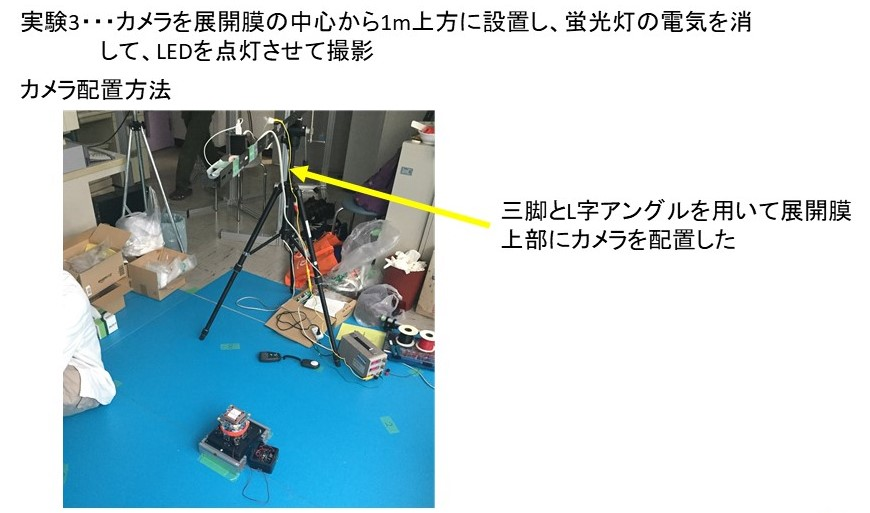
\includegraphics[width=.9\textwidth]{03/fig/3-9-2-3-1.jpg}
	\caption{三脚上に設置した伸展カメラ部BBMによる膜展開撮影の実験構成}
	\label{fig3-9-2-3-1}
\end{figure}
\begin{figure}[H]
	\centering
	\begin{tabular}{cc}
		\begin{minipage}{0.5\hsize}
			\begin{center}
				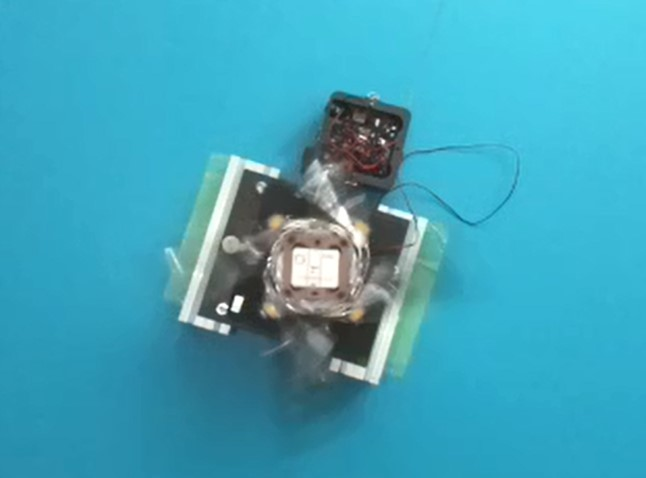
\includegraphics[width=1\textwidth]{03/fig/3-9-2-3-2.jpg}
			\end{center}
		\end{minipage}&
		\begin{minipage}{0.5\hsize}
			\begin{center}
				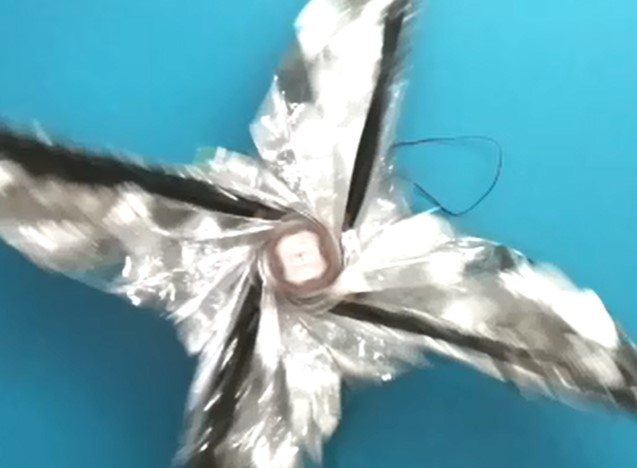
\includegraphics[width=1\textwidth]{03/fig/3-9-2-3-3.jpg}
			\end{center}
		\end{minipage}\\
		\begin{minipage}{0.5\hsize}
			\begin{center}
				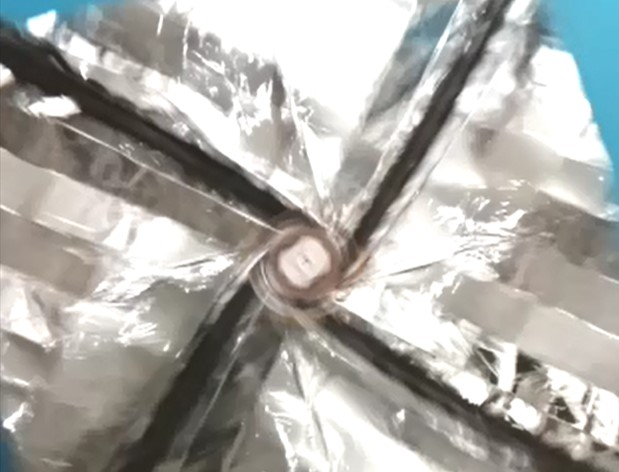
\includegraphics[width=1\textwidth]{03/fig/3-9-2-3-4.jpg}
			\end{center}
		\end{minipage}&
		\begin{minipage}{0.5\hsize}
			\begin{center}
				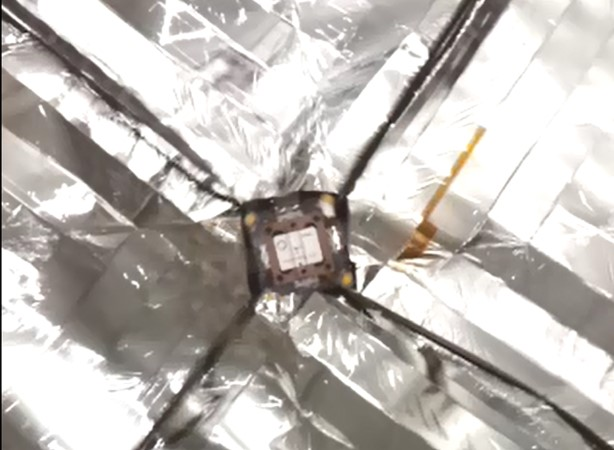
\includegraphics[width=1\textwidth]{03/fig/3-9-2-3-5.jpg}
			\end{center}
		\end{minipage}
	\end{tabular}
	\caption{三脚上に設置した伸展カメラ部BBMによる膜展開撮影結果}
	\label{fig3-9-2-3-2}
\end{figure}

\noindent \textbf{2017/04/18 伸展マスト付き織物膜(EM1)展開撮影実験}
\begin{itemize}
	\item 古谷研にて実施.参加者:東工大古谷研、坂本研、首都大鳥阪、西井、ISAS名取、奥泉、佐藤(敬称略).実験の詳細は膜展開部の項で述べる.
	\item 膜上のデバイスもダミーを設置した(ただしハーネスはなし).1mブームの上部に伸展カメラ部BBMを天井から吊り下げて設置した.伸展カメラ部に伸びるハーネスもダミーを取り付けた.広角レンズを使用.
	\item 部屋の蛍光灯をONした状態で展開.40fpsに落として,撮影画角を広くしたところ,全体の展開動画が撮影できた.
	\item 課題: 照明条件と反射マーカーを模擬した上で,暗闇の中での撮影可能性を検証する必要がある.→この実験後,SDDL暗室内でLED+マーカーを動画撮影し,撮影できる見込みを得てEM製作を実施した.
\end{itemize}
\begin{figure}[H]
	\centering
	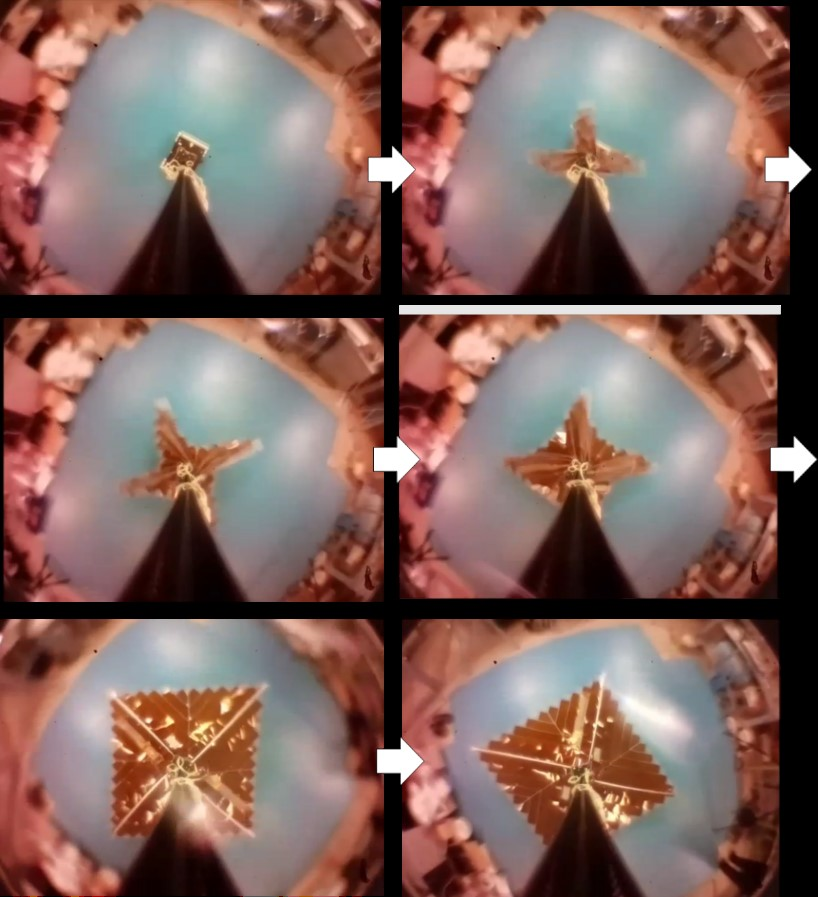
\includegraphics[width=.8\textwidth]{03/fig/3-9-2-3-6.jpg}
	\caption{伸展マスト付き織物膜(EM1)展開撮影結果}
	\label{fig3-9-2-3-6}
\end{figure}

\noindent \textbf{2018/04/23 暗室での織物膜(EM2)動画撮影試験}
\begin{itemize}
	\item 古谷研にて実施.窓を暗幕でふさぎ,照明をOFFして暗闇の中で実験した.床からの照り返しを避けるため,床にも暗幕を敷いた.
	\item FMとほぼ同じ仕様でマーカーを貼り付けたEM2膜の展開時,および展張後に,膜から高さ1mに吊り下げた伸展カメラ部BBMからのLEDの照明のみで動画撮影を行った.
	\item 綺麗に展開の動画が撮影できた.ただ照明がやや強すぎる(マーカーが光りすぎている)と考え,開いた後の膜を手で揺らしながら,LEDの明るさを徐々に暗くして適切な明るさへ調整した.
\end{itemize}
\begin{figure}[H]
	\centering
	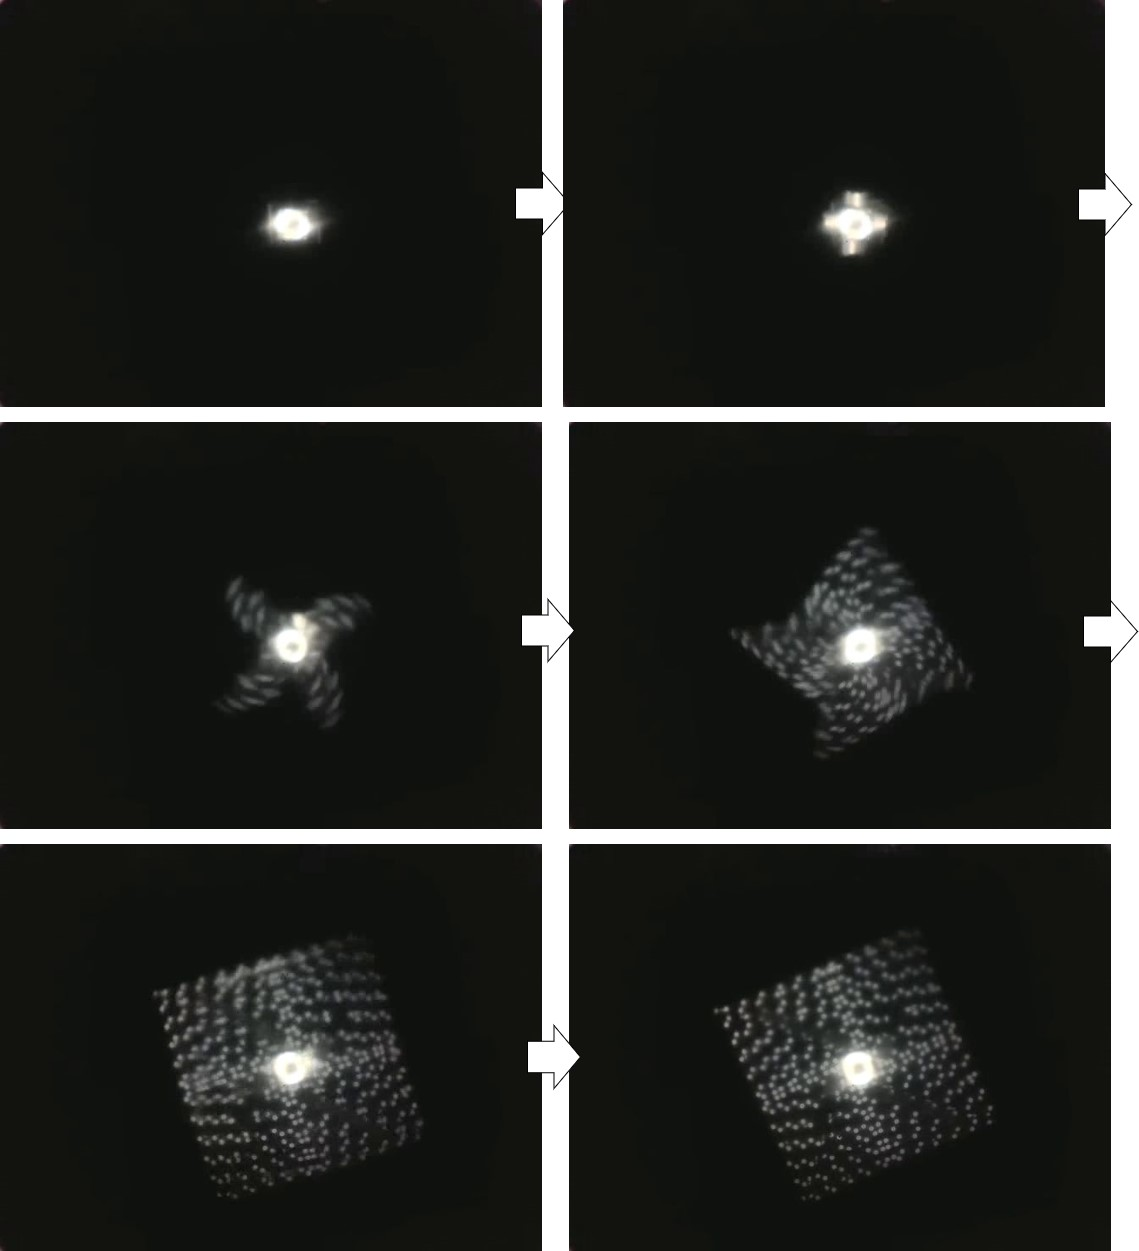
\includegraphics[width=.8\textwidth]{03/fig/3-9-2-3-7.jpg}
	\caption{伸展カメラ部LED照明織物膜(EM2)展開撮影結果}
	\label{fig3-9-2-3-7}
\end{figure}


\subsubsection{切り離し試験(ウェルリサーチ・坂本)}

伸展マストを根元から切り離す,切り離し機構を以下のように検証した.まず,伸展マストに沿って引き出されたハーネスのコネクタを留めるテグスが溶断される.
コネクタは図\ref{fig3-9-2-1-4}のようになっており,ブームの伸展を続けることで引き抜かれる.図\ref{fig3-9-2-1-5}に示すコンフィグレーションの試験でEM設計の妥当性を確認した.
\begin{figure}[H]
	\centering
	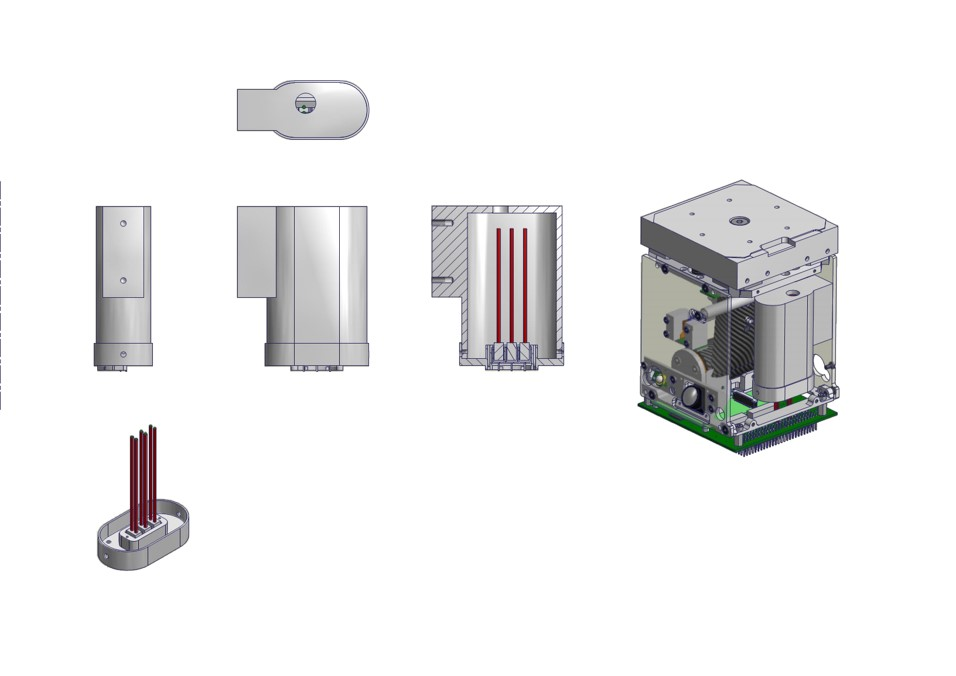
\includegraphics[width=.7\textwidth]{03/fig/3-9-2-1-4.jpg}
	\caption{伸展マスト部のケーブルボックス}
	\label{fig3-9-2-1-4}
\end{figure}
\begin{figure}[H]
	\centering
	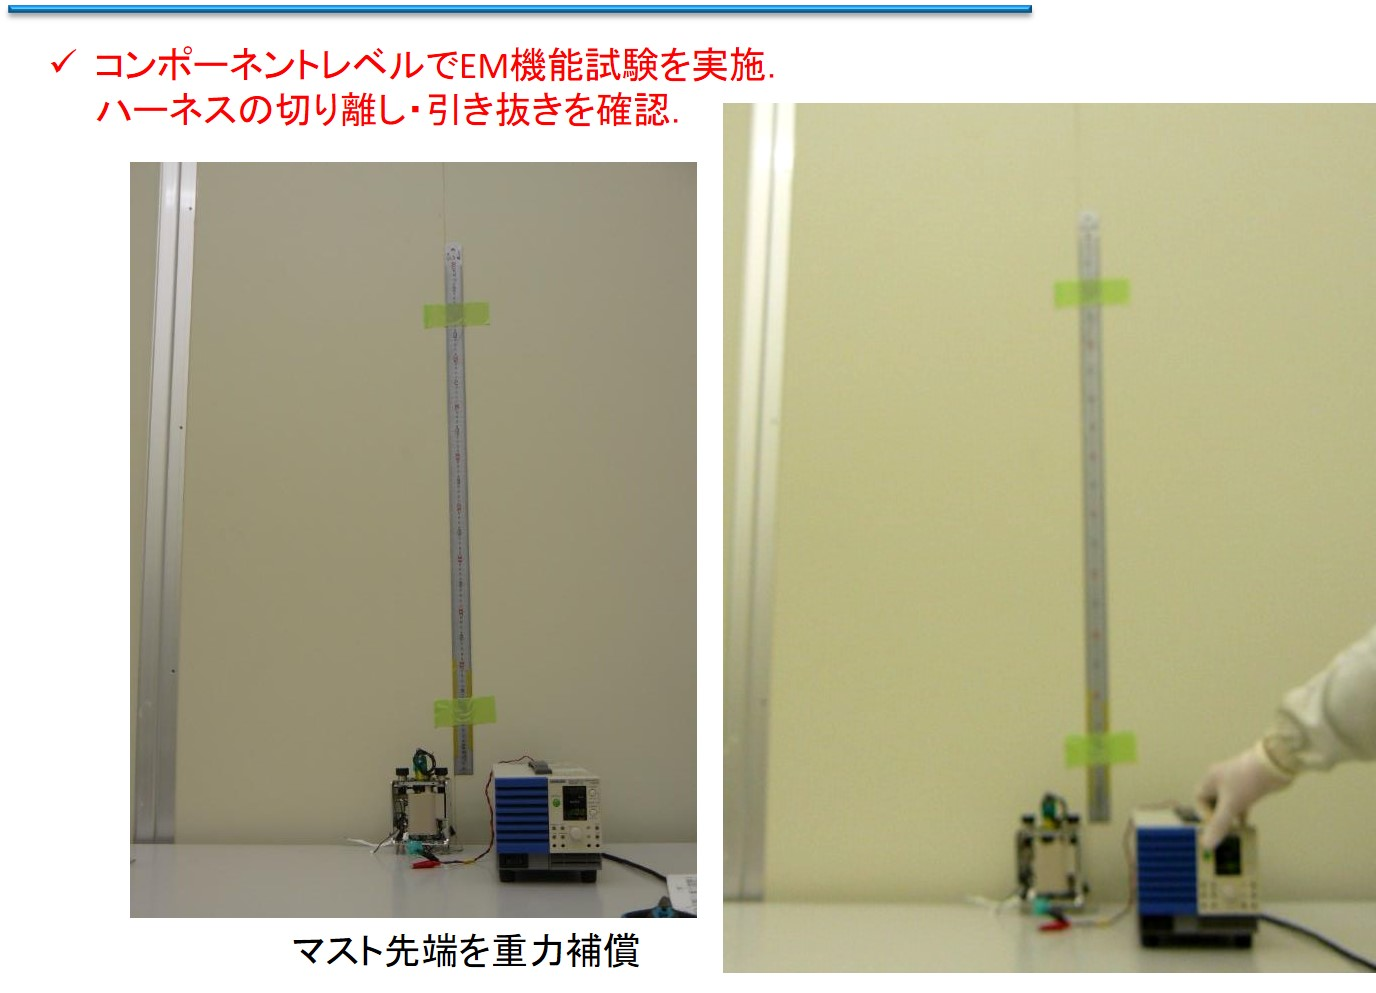
\includegraphics[width=.8\textwidth]{03/fig/3-9-2-1-5.jpg}
	\caption{伸展マストのコネクタの引き抜き試験}
	\label{fig3-9-2-1-5}
\end{figure}

ブーム根元を切り離す試験については,図\ref{fig3-9-2-1-6}での試験を実施したがじゅうぶんなブーム根元の飛び出しを確認できなかったため,さらに捩りばねを改良して最終的な設計に到達した.
切り離しを確認した試験の様子を図\ref{fig3-9-2-1-7}に示す.
\begin{figure}[H]
	\centering
	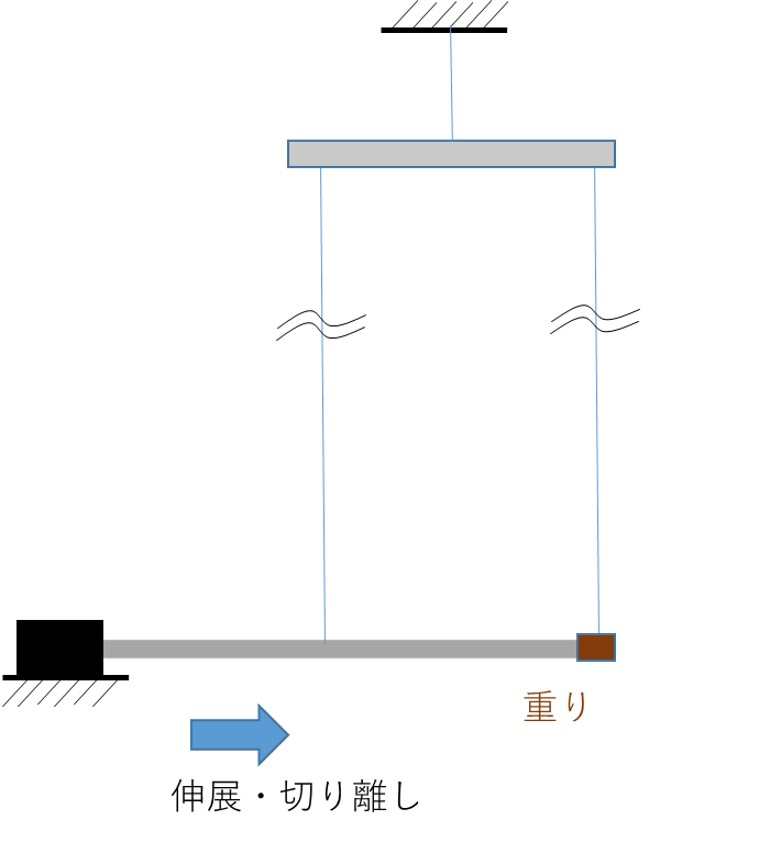
\includegraphics[width=.4\textwidth]{03/fig/3-9-2-1-6.jpg}
	\caption{伸展マストのブーム切り離し試験コンフィグレーション}
	\label{fig3-9-2-1-6}
\end{figure}
\begin{figure}[H]
	\centering
	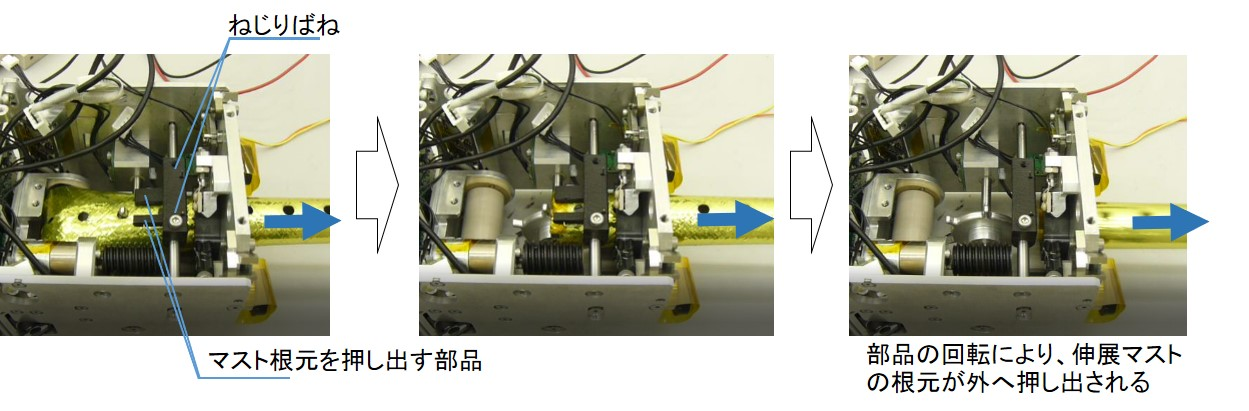
\includegraphics[width=.8\textwidth]{03/fig/3-9-2-1-7.jpg}
	\caption{伸展マストのブーム切り離し試験}
	\label{fig3-9-2-1-7}
\end{figure}
